\section{Build Project with Make}
\label{sec:make}
\begin{frame}<beamer>
    \frametitle{Outline}
    \tableofcontents[currentsection]
\end{frame}

\begin{frame}[fragile]{Why make? (1)}
\vspace{-0.3in}
\begin{columns}
\begin{column}{0.4\linewidth}
\begin{lstlisting}{mylib.h}}[linewidth=0.9\linewidth]
#ifndef MYLIB_H
#define MYLIB_H
int isodd(int x);
float square(float x);
#endif
\end{lstlisting}
\vspace{-0.1in}
\begin{lstlisting}{mylib.c}[linewidth=0.9\linewidth]
#include "mylib.h"
float square(float x){
    return x*x;
}

int isodd(int x){
    if(x%2 != 0)
      return 1;
    else
      return 0;
}
\end{lstlisting}
\end{column}
\begin{column}{0.54\linewidth}
\begin{lstlisting}{main.c}
#include "mylib.h"
#include <stdio.h>
int main(){
  float x = 3.4;
  int a = 5;
  float y = square(x);
  if(isodd(a))
  {
       printf("%d is odd\n", a);
  }
  return 0;
}
\end{lstlisting}
\vspace{-0.15in}
\begin{lstlisting}{Build the project}[language=make]
gcc myproj.c -o myproj.o -c
gcc mylib.c -o mylib.o -c

gcc -o myproj myproj.o mylib.o
\end{lstlisting}
\end{column}
\end{columns}
\end{frame}

\begin{frame}[fragile]{Why make? (2)}

\begin{lstlisting}[language=make, linewidth=0.75\linewidth, firstnumber=1,caption="Build the project"]
gcc myproj.c -o myproj.o -c
gcc mylib.c -o mylib.o -c

gcc -o myproj myproj.o mylib.o
\end{lstlisting}
\begin{itemize}
	\item {In practice, we may have many libraries to compile and link}
	\vspace{0.15in}
	\item {\textcolor{red}{gcc} -o \textcolor{green}{myproj} myproj.o mylib.o}
	\vspace{0.15in}
	\item {If we do it manually, it is too laborious!!!}
\end{itemize}

\begin{itemize}
	\item {This is where ``Makefile'' comes to fit in}
\end{itemize}
\end{frame}

\begin{frame}{Makefile}
\begin{itemize}
	\item {A script file organize all the compilation things together}
		\vspace{0.15in}
	\item {It is responsible for}
		\vspace{0.15in}
		\begin{enumerate}
			\item {Compiling the source files (compile from \textcolor{red}{.c} to  \textcolor{red}{.o})}
			\vspace{0.15in}
			\item {Linking the files into the final executable software}
			\vspace{0.15in}
			\item {Installing the software to target directory}
		\end{enumerate}
		\item {Command \textcolor{red}{make} will parse the script}
		\item {It fulfills the intructions in the script}
\end{itemize}
\end{frame}

\begin{frame}[fragile]{Prepare Environment (1)}
\begin{itemize}
	\item {Define the variables}
\end{itemize}
\lstset{language=[gnu] make}
\lstset{
   language=[gnu] make,
   keywordstyle=\color{teal}\textbf,
   stringstyle=\color{blue},
   identifierstyle=\itshape
}
\begin{lstlisting}[linewidth=0.9\linewidth, xleftmargin=0.05\linewidth]
WORK_DIR=.
CC=gcc
LD=gcc
OBJ_DIR=$(WORK_DIR)/obj
OBJ_RELEASE=$(OBJ_DIR)/mylib.o $(OBJ_DIR)/myproj.o
RELEASE=$(WORK_DIR)/bin/myproj
\end{lstlisting}

\begin{itemize}
	\item {command \textcolor{red}{make} supports environment variable definitions }
\end{itemize}
\begin{center}
	\Large{VARIABLE\_NAME = value}
\end{center}
\begin{itemize}
	\item {One can specify the file, directory, command, compilation parameters}
	\item {They may support the compilation of the project}
\end{itemize}
\end{frame}


\begin{frame}[fragile]{Prepare Environment (2)}
\lstset{
   language=[gnu] make,
   keywordstyle=\color{teal}\textbf,
   stringstyle=\color{blue},
   identifierstyle=\itshape
}
\begin{lstlisting}[linewidth=0.9\linewidth, xleftmargin=0.05\linewidth]{Makefile}
WORK_DIR=.
CC=gcc
LD=gcc
\end{lstlisting}
\vspace{-0.2in}
\begin{itemize}
	\item {Command \textcolor{red}{make} supports environment variable definitions }
\end{itemize}
\begin{center}
	\Large{WORK\_DIR = .}
\end{center}
\begin{itemize}
	\item {Specify the project directory where ``Makefile'' and the project is located}
	\item {The  variable name is by convention \textcolor{red}{CAPITALIZED}}
\end{itemize}
\end{frame}

\begin{frame}[fragile]{Prepare Environment (3)}
\lstset{language=[gnu] make}
\lstset{
   language=[gnu] make,
   keywordstyle=\color{teal}\textbf,
   stringstyle=\color{blue},
   identifierstyle=\itshape
}
\begin{lstlisting}[linewidth=0.9\linewidth, xleftmargin=0.05\linewidth, caption=Makefile]
WORK_DIR=.
CC=gcc
LD=gcc
\end{lstlisting}
\vspace{-0.2in}
\begin{itemize}
	\item {Command \textcolor{red}{make} supports environment variable definitions }
\end{itemize}
\begin{center}
	\Large{CC=gcc}\\
	\Large{LD=gcc}
\end{center}
\begin{itemize}
	\item {``CC=gcc'' specifies the compiler}
	\item {``LD=gcc'' specifies the linker}
\end{itemize}
\end{frame}

\begin{frame}[fragile]{Prepare Environment (4)}
\vspace{-0.2in}
\lstset{language=[gnu] make}
\lstset{
   language=[gnu] make,
   keywordstyle=\color{teal}\textbf,
   stringstyle=\color{blue},
   identifierstyle=\itshape
}
\begin{lstlisting}[linewidth=0.9\linewidth, xleftmargin=0.05\linewidth, caption=Makefile]
OBJ_DIR=$(WORK_DIR)/obj
OBJ_RELEASE=$(OBJ_DIR)/mylib.o $(OBJ_DIR)/myproj.o
RELEASE=$(WORK_DIR)/bin/myproj
\end{lstlisting}
\vspace{-0.2in}
\begin{itemize}
	\item {Command \textcolor{red}{make} supports environment variable definitions }
\end{itemize}
\begin{center}
	\Large{\$(WORK\_DIR)/obj}
\end{center}
\vspace{-0.2in}
\begin{itemize}
	\item {\$(VARIABLE) cite the value of the VARIABLE}
	\item {Here ``\$(WORK\_DIR)'' is replaced by ``./''}
\end{itemize}
\end{frame}


\begin{frame}[fragile]{Prepare Environment (5)}
\vspace{-0.2in}
\lstset{language=[gnu] make}
\lstset{
   language=[gnu] make,
   keywordstyle=\color{teal}\textbf,
   stringstyle=\color{blue},
   identifierstyle=\itshape
}
\begin{lstlisting}[linewidth=0.9\linewidth, xleftmargin=0.05\linewidth, caption=Makefile]
OBJ_DIR=$(WORK_DIR)/obj
OBJ_RELEASE=$(OBJ_DIR)/mylib.o $(OBJ_DIR)/myproj.o
RELEASE=$(WORK_DIR)/bin/myproj
\end{lstlisting}
\vspace{-0.1in}
\begin{itemize}
	\item {The above instructions indicate}
	\begin{enumerate}
		\item {The object files will be put to \textcolor{red}{./obj/}}
		\item {``OBJ\_RELEASE'' keeps the lists of all object files}
		\item {The final target binary software name is ``myproj''}
		\item {It will be put to \textcolor{red}{./bin/}}
	\end{enumerate}
\end{itemize}

\end{frame}


\begin{frame}[fragile]{Prepare Environment (6)}
\lstset{language=[gnu] make}
\lstset{
   language=[gnu] make,
   keywordstyle=\color{teal}\textbf,
   stringstyle=\color{blue},
   identifierstyle=\itshape
}
\begin{lstlisting}[linewidth=0.9\linewidth, xleftmargin=0.05\linewidth]
WORK_DIR=.
CC=gcc
LD=gcc
OBJ_DIR=$(WORK_DIR)/obj
OBJ_RELEASE=$(OBJ_DIR)/mylib.o $(OBJ_DIR)/myproj.o
RELEASE=$(WORK_DIR)/bin/myproj
\end{lstlisting}

\begin{enumerate}
	\item {We know the working directory }
	\item {We have the compiler and linker}
	\item {We know where we should put the object files}
	\item {We know where we should put the target binary file}
\end{enumerate}
\end{frame}

\begin{frame}[fragile]{Prepare Environment (7)}
\lstset{language=[gnu] make}
\lstset{
   language=[gnu] make,
   keywordstyle=\color{teal}\textbf,
   stringstyle=\color{blue},
   identifierstyle=\itshape
}
\begin{lstlisting}[linewidth=0.9\linewidth, xleftmargin=0.05\linewidth]
WORK_DIR=.
CC=gcc
LD=gcc
OBJ_DIR=$(WORK_DIR)/obj
OBJ_RELEASE=$(OBJ_DIR)/mylib.o $(OBJ_DIR)/myproj.o
RELEASE=$(WORK_DIR)/bin/myproj

before_release:
        test -d bin || mkdir -p bin
        test -d $(OBJ_DIR) || mkdir -p $(OBJ_DIR)
\end{lstlisting}

\begin{enumerate}
	\item {However, ``./obj/'' and ``./bin/'' are not ready }
	\item {We can test and make them if necessary}
\end{enumerate}
\end{frame}

\begin{frame}[fragile]{Compile the source file}
\lstset{language=[gnu] make}
\lstset{
   language=[gnu] make,
   keywordstyle=\color{teal}\textbf,
   stringstyle=\color{blue},
   identifierstyle=\itshape
}
\begin{lstlisting}[linewidth=0.9\linewidth, xleftmargin=0.05\linewidth]
$(OBJ_DIR)/mylib.o: mylib.c
        $(CC) -c mylib.c -o $(OBJ_DIR)/mylib.o
\end{lstlisting}
\vspace{-0.15in}
\begin{itemize}
	\item {Instruction ``\$(OBJ\_DIR)/mylib.o'' compiles ``mylib.c''}
	\item {The compilation relies on file ``mylib.c''}
	\item {The indentation should  be by ``Tab''}
	\item {We can do so for all the source files}
	\item {The resulting file is put to ``./obj/mylib.o'' }
\end{itemize}
\begin{lstlisting}[linewidth=0.9\linewidth, xleftmargin=0.05\linewidth]
$(OBJ_DIR)/mylib.o: mylib.c
        $(CC) -c mylib.c -o $(OBJ_DIR)/mylib.o
        
$(OBJ_DIR)/myproj.o: myproj.c
        $(CC) -c myproj.c -o $(OBJ_DIR)/myproj.o
\end{lstlisting}
\end{frame}

\begin{frame}[fragile]{Link the source file}
\lstset{language=[gnu] make}
\lstset{
   language=[gnu] make,
   keywordstyle=\color{teal}\textbf,
   stringstyle=\color{blue},
   identifierstyle=\itshape
}
\begin{lstlisting}[linewidth=0.9\linewidth, xleftmargin=0.05\linewidth]
release: $(OBJ_RELEASE)
        $(LD) -o $(RELEASE) $(OBJ_RELEASE)
\end{lstlisting}
\vspace{-0.15in}
\begin{itemize}
	\item {The project will be linked with mylib.o and myproj.o}
	\item {The list of object files are kept in ``\$(OBJ\_RELEASE)''}
	\item {\$(LD) calls ``gcc''}
	\item {The target is specified by ``\$(RELEASE)''}
\end{itemize}

\end{frame}

\begin{frame}[fragile]{Build the whole project}
\lstset{language=[gnu] make}
\lstset{
   language=[gnu] make,
   keywordstyle=\color{teal}\textbf,
   stringstyle=\color{blue},
   identifierstyle=\itshape
}
\begin{lstlisting}[linewidth=0.9\linewidth, xleftmargin=0.05\linewidth]
release: before_release $(OBJ_RELEASE)
        $(LD) -o $(RELEASE) $(OBJ_RELEASE)
\end{lstlisting}
\vspace{-0.15in}
\begin{itemize}
	\item {The instruction ``release''  relies on another two intructions}
	\item {``before\_release'' and ``\$(OBJ\_RELEASE)''}
	\item {``\$(OBJ\_RELEASE)'' are a list of instructions}
	\begin{enumerate}
		\item {Run instruction ``before\_release''}
		\item {Run list of instructions in ``\$(OBJ\_RELEASE)''}
		\item {Run \$(LD) -o \$(RELEASE) \$(OBJ\_RELEASE)}
	\end{enumerate}
\end{itemize}

\end{frame}


\begin{frame}[fragile]{Clean the object files}
\lstset{language=[gnu] make}
\lstset{
   language=[gnu] make,
   keywordstyle=\color{teal}\textbf,
   stringstyle=\color{blue},
   identifierstyle=\itshape
}
\begin{itemize}
	\item {In some cases, we may want to clean the object files}
\end{itemize}
\begin{lstlisting}[linewidth=0.9\linewidth, xleftmargin=0.05\linewidth]
clean:
        rm -rf $(OBJ_DIR)/*.o
        rm -rf $(RELEASE)
\end{lstlisting}
\vspace{-0.15in}
\begin{itemize}
	\item {We call command ``rm''}
	\item {We label the instruction as ``clean''}
\end{itemize}

\end{frame}

\begin{frame}[fragile]{A Complete Makefile}
\vspace{-0.2in}
\lstset{language=[gnu] make}
\lstset{
   language=[gnu] make,
   keywordstyle=\color{teal}\textbf,
   stringstyle=\color{blue},
   identifierstyle=\itshape
}
\begin{lstlisting}[linewidth=0.9\linewidth, xleftmargin=0.05\linewidth]{Makefile}
WORK_DIR=.
CC=gcc
LD=gcc
OBJ_DIR=$(WORK_DIR)/obj
OBJ_RELEASE=$(OBJ_DIR)/mylib.o $(OBJ_DIR)/myproj.o
RELEASE=$(WORK_DIR)/bin/myproj

$(OBJ_DIR)/mylib.o: mylib.c
        $(CC) -c mylib.c -o $(OBJ_DIR)/mylib.o

$(OBJ_DIR)/myproj.o: myproj.c
        $(CC) -c myproj.c -o $(OBJ_DIR)/myproj.o

before_release:
        test -d bin || mkdir -p bin
        test -d $(OBJ_DIR) || mkdir -p $(OBJ_DIR)

release: before_release $(OBJ_RELEASE)
        $(LD) -o $(RELEASE) $(OBJ_RELEASE)
\end{lstlisting}

\end{frame}

\begin{frame}[fragile]{A Complete Makefile}

\begin{lstlisting}[linewidth=0.9\linewidth, xleftmargin=0.05\linewidth]{Makefile}
clean:
        rm -rf $(OBJ_DIR)/*.o
        rm -rf $(RELEASE)
\end{lstlisting}
\begin{itemize}
	\item {Five major sections}
	\begin{enumerate}
		\item {Define the environment variables}
		\item {Prepare directories}
		\item {Instructions of compiling source files to object files}
		\item {Link object files to target binary executable or library}
		\item {Instructions to clean the object files}
	\end{enumerate}
\end{itemize}
\end{frame}


\begin{frame}{Running Flow inside Makefile (1)}
\begin{figure}
	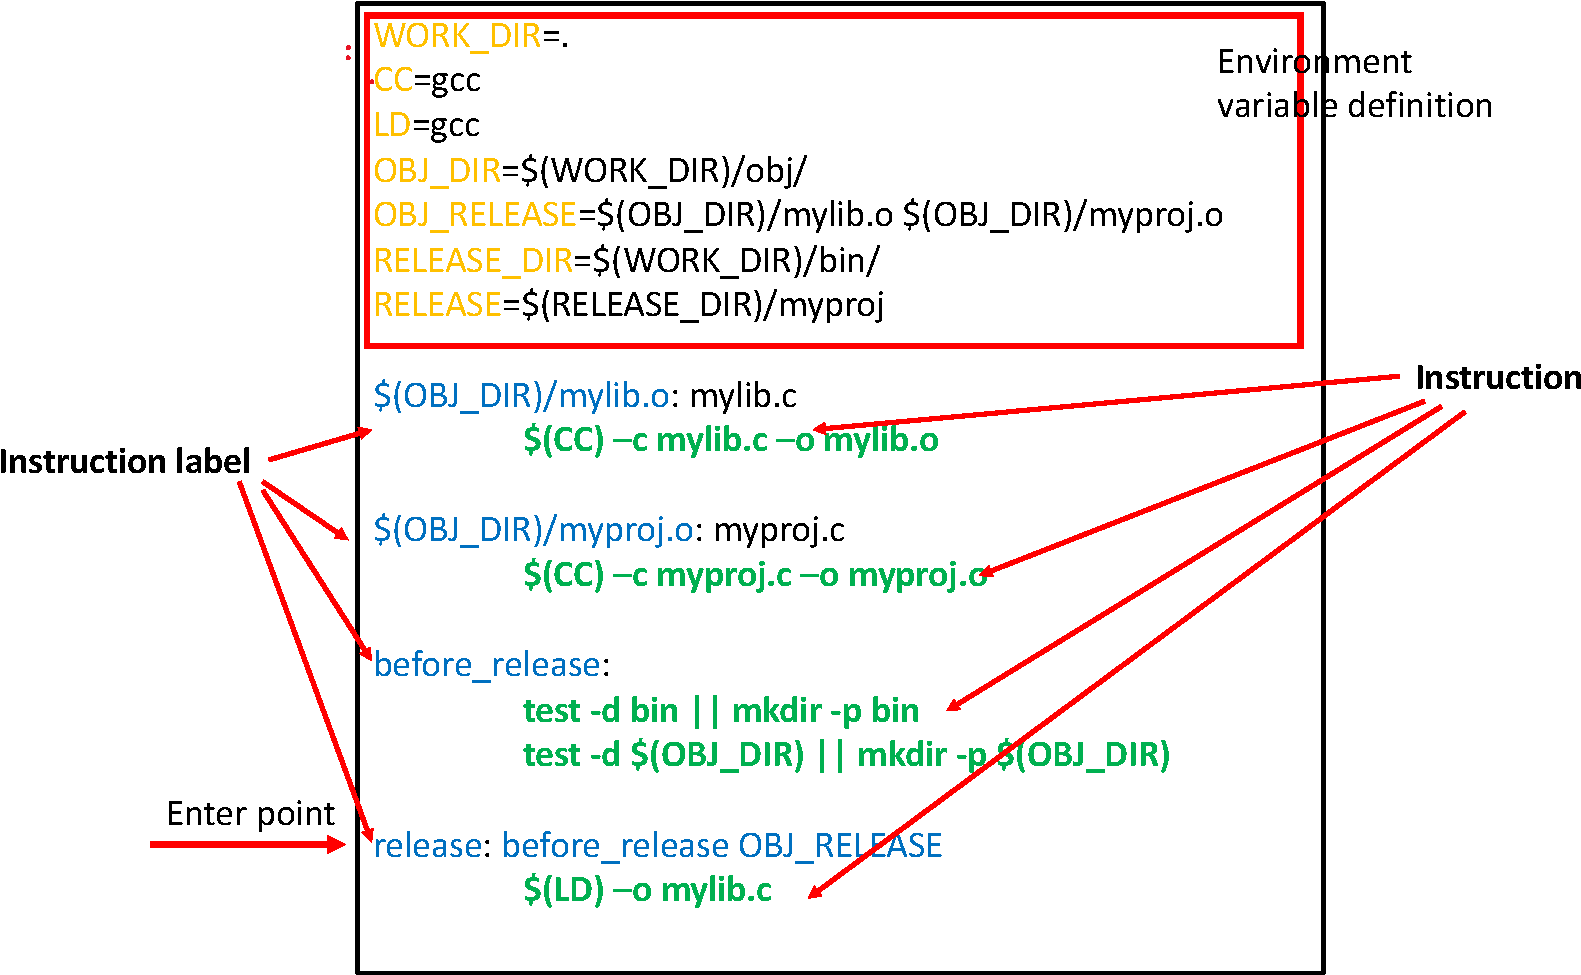
\includegraphics[width=0.80\linewidth]{figs/make1.pdf}
\end{figure}
\begin{itemize}
	\item {Run command ``\textcolor{blue}{make release}''}
\end{itemize}
\end{frame}

\begin{frame}{Running Flow inside Makefile (2)}
\begin{figure}
	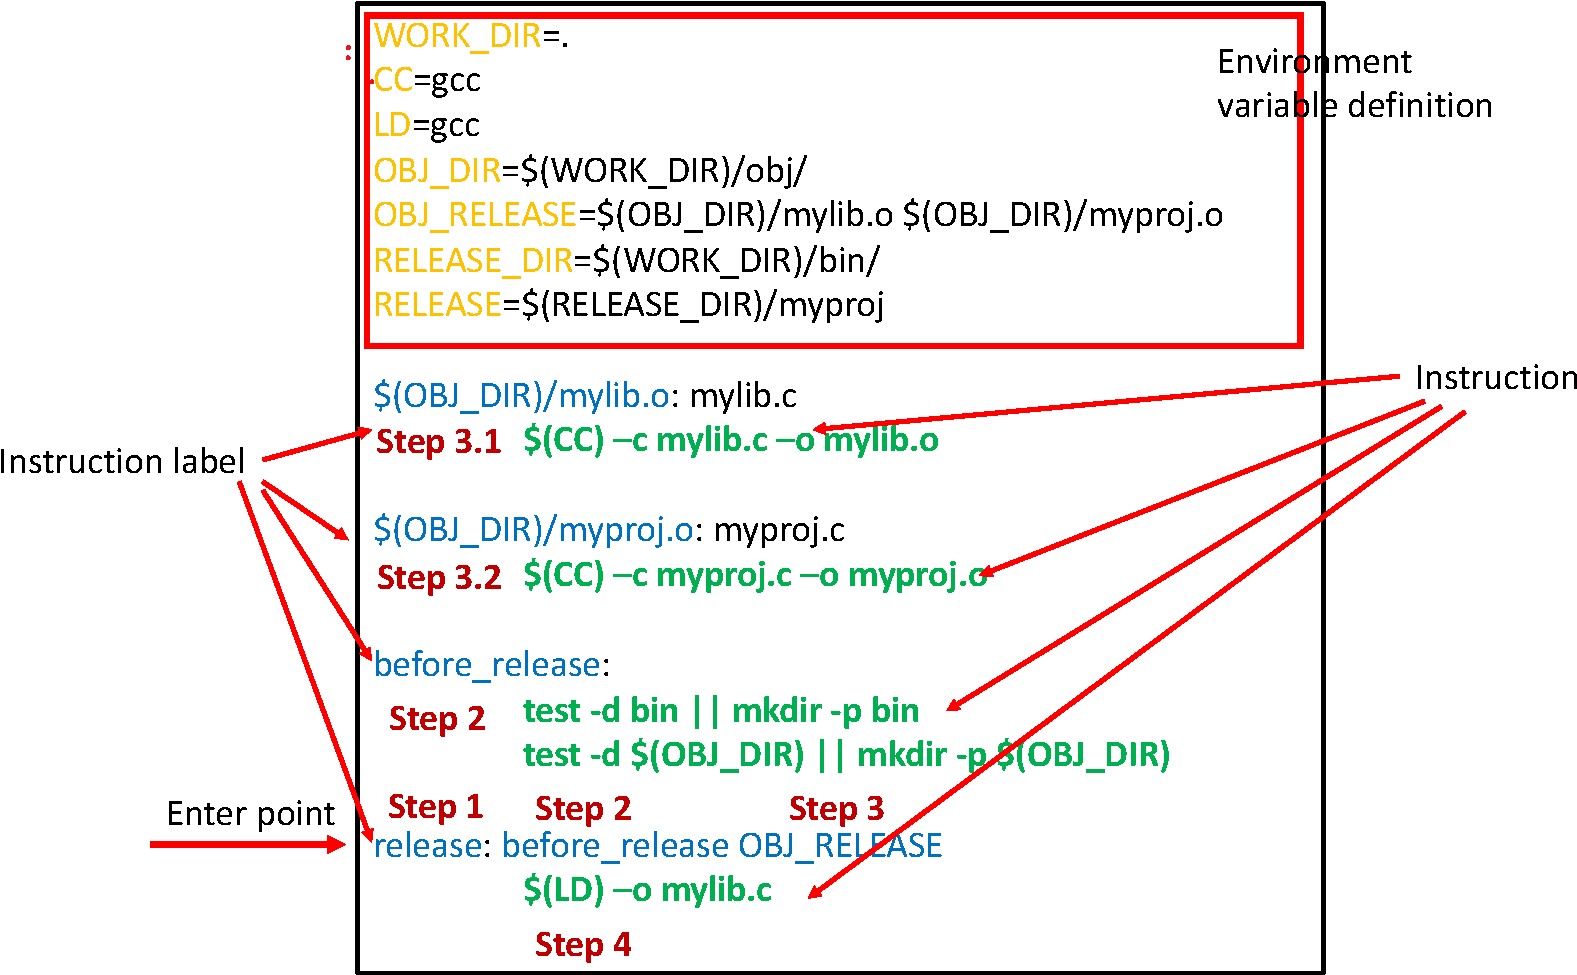
\includegraphics[width=0.80\linewidth]{figs/make2.pdf}
\end{figure}
\begin{itemize}
	\item {Run command ``\textcolor{blue}{make release}''}
\end{itemize}
\end{frame}

\begin{frame}[fragile]{Add libraries in Makefile (1)}
\begin{itemize}
	\item {We may need either static or dynamic libraries or both}
\end{itemize}
\begin{lstlisting}[linewidth=0.9\linewidth, firstnumber=1, xleftmargin=0.05\linewidth]{myproj.c}
#include <math.h>
#include "mylib.h"
#include <stdio.h>
int main(){
  float x = 3.4;
  int a = 5;
  float y = square(x);
  float z = sqrt(x);
  return 0;
}
\end{lstlisting}
\begin{itemize}
	\item {For this code, we should compile it by}
\end{itemize}
\begin{lstlisting}[linewidth=0.9\linewidth, xleftmargin=0.05\linewidth]
gcc -o myproj myproj.o mylib.o -lm
\end{lstlisting}
\end{frame}

\begin{frame}[fragile]{Add libraries in Makefile (2)}
\vspace{-0.2in}
\begin{lstlisting}[linewidth=0.95\linewidth, firstnumber= 1, xleftmargin=0.02\linewidth]{Makefile}
WORK_DIR=.
CC=gcc
LD=gcc
LDFLAGS= -lm
OBJ_DIR=$(WORK_DIR)/obj
OBJ_RELEASE=$(OBJ_DIR)/mylib.o $(OBJ_DIR)/myproj.o
RELEASE=$(WORK_DIR)/bin/myproj

$(OBJ_DIR)/mylib.o: mylib.c
        $(CC) -c mylib.c -o $(OBJ_DIR)/mylib.o

$(OBJ_DIR)/myproj.o: myproj.c
        $(CC) -c myproj.c -o $(OBJ_DIR)/myproj.o

before_release:
        test -d bin || mkdir -p bin
        test -d $(OBJ_DIR) || mkdir -p $(OBJ_DIR)

release: before_release $(OBJ_RELEASE)
        $(LD) $(LDFLAGS) -o $(RELEASE) $(OBJ_RELEASE)
\end{lstlisting}

\end{frame}
